O sistema físico escolhido para a realização deste trabalho
consiste basicamente em uma aplicação genérica de controle de motor de 
corrente contínua através de modulação por largura de pulso, 
e a utilização de um controlador de 32-bits, núcleo ARM, 
de forma a explorar o controlador utilizado como suporte ao 
curso que gerou esta pesquisa. A importância do sistema eletrônico se faz 
pelo caráter demostrativo que se tem na proposta do projeto, 
para garantir uma veracidade às proposições feitas com a 
nova ferramenta abordada, a LPA2v, 
e validar de forma física e mensurável os dados e resultados.



\section{Atuador}

O motor elétrico é um dos dispositivos 
conversores de energia mais utilizados nos 
diversos meios tecnológicos, 
estando presentes largamente na indústria, 
em equipamentos eletrodomésticos, 
eletrônicos, automóveis, smarthphones, 
e uma variedade enorme de aplicações. 

Os motores elétricos podem ser divididos em dois grandes grupos, 
em função do tipo de alimentação que utilizam, e são eles 
motores de corrente alternada, 
cuja velocidade pode ser controlada pela mudança da frequência e 
motores de corrente contínua, 
que basta alterar o nível de tensão para haver uma variação da velocidade, 
e no caso de motores de pequeno porte, 
são mais utilizados pela facilidade do seu controle. 

O motor de corrente contínua (motor CC) \nomenclature{CC}{Corrente Contínua}%
é composto por uma parte fixa e outra móvel, 
denominadas respectivamente de Estator e Rotor. 
Seu princípio de funcionamento basicamente acontece pela 
relação de interação entre as forças eletromagnéticas. 
Uma bobina de fio é atravessada por um campo magnético 
gerado por ímãs fixos. 
Ao aplicar uma corrente elétrica na bobina, 
esta gera um campo elétrico que interage com o campo magnético, 
gerando uma força de rotação, ou Torque, que faz o eixo girar. 
Quando a bobina, 
que forma o eixo de rotação se desloca até um determinado limite, 
seus terminais comutam e trocam de polaridade, 
mantendo os polos de interação sempre gerando a força de torção no eixo. 
O elemento que faz a troca de polaridade na bobina é denominado comutador.

A velocidade de rotação do eixo depende 
da intensidade do campo elétrico gerado pela bobina 
e que interage com o campo magnetico gerada pelos ímãs fixos, 
assim, quanto maior for o campo gerado 
maior será a velocidade, 
e a intensidade do campo elétrico depende da 
intensidade de corrente que circula pela bobina, 
e esta depende da tensão aplicada aos teminais. 
Logo, alterando a tensão aplicada, altera-se a corrente, 
por consequência o campo elétrico e também a velocidade de rotação do motor.

A Figura  \ref{fig:motorDC} mostra o motor CC utilizado no estudo mostrado neste trabalho, 
sendo um motor de baixa potência e baixo torque, mas de alta velocidade. 


\begin{figure}[!htb]
\caption{Motor CC}
\center\includegraphics[scale=0.1, angle=0, clip=true, trim=1500 500 400 200]{./imagens/motorDC.jpg}
\label{fig:motorDC}

{\small Fonte: Próprio autor}
\end{figure}

Para alimentação do motor, 
assim como do restante do sistema foi utilizada uma fonte chaveada de saída 12Vcc.


O motor foi fixado a uma base de plástico com um furo contendo a medida de seu diâmetro, 
de forma a não haver folga e garantir uma estabilidade do motor 
sobre a superfície de repouso do sistema.

Para gerar alguma carga, 
foi utilizado um CD acoplado ao eixo do motor, de forma centralizada 
e foi utilizada uma etiqueta de plástico presa na borda do CD \nomenclature{CD}{\emph{Compact Disc}}%
para formar um ponto de leitura pelo sensor óptico, 
como se vê na Figura \ref{fig:discoSensor}.

\section{Sensor}

Para a leitura de velocidade foi utilizado 
um conjunto de sensor óptico para reconhecer cada giro do disco, 
e poder mensurar a velocidade de rotação do motor.

A Figura \ref{fig:discoSensorGeral} mostra uma visão geral do sistema montado, 
utilizando o motor e o sensor posicionados de 
forma a serem feitas as experiências e testes pertinentes ao estudo.

\begin{figure}[!htb]
\center
\caption{Visão geral do sistema }
\subfloat[]{
	\label{fig:discoSensor}
	\includegraphics[scale=0.07, angle=0, clip=true, trim=300 200 1200 200]{./imagens/discoSensor.jpg}
	}
\subfloat[]{ 
	\label{fig:discoSensorGeral} 
	\includegraphics[scale=0.07, angle=0, clip=true, trim=300 200 400 200]{./imagens/discoSensorGeral.jpg} 
	}

{ \small Fonte: Próprio autor}
\end{figure}





\section{Drive}

Para controlar a velocidade do motor cc, 
é necessário alterar a tensão aplicada nele, 
e a técnica mais comum é a 
Modulação por Largura de Pulso (do inglês: \emph{Pulse Width Modulation - PWM}, \nomenclature{PWM}{Pulse Width Modulation}%
que consiste em chavear a alimentação a uma frequência fixa mas modulando, 
ou seja, alterando a largura dos pulsos, 
de forma que a tensão média aplicada possa ser controlada e 
o motor tenha uma alimentação que varia de zero até o valor da fonte 
para os respectivos valores de PWM.

\begin{figure}[!htb]
\caption{Drive}
\center\includegraphics[scale=0.1, angle=0, clip=true, trim=0 0 0 0]{./imagens/drive.jpg}
\label{fig:drive}
{ \small Fonte: Próprio autor}
\end{figure}

Como elemento de acionamento do motor foi utilizado um transistor tipo MOS 
\nomenclature{MOS}{Metal Oxide Semiconductor}%
e um optoacoplador para isolar o acionamento do motor do controlador.

\section{Controlador}

Para o estudo proposto foi utilizado uma placa de desenvolvimento da Texas Instruments de modelo Tiva$^{TM}$ TM4C123GH6PM. A sua escolha deveu-se ao fato de que ela possui um controlador de 32bits, núcleo ARM.

\begin{itemize}
\item Núcleo (Core): ARM Cortex-M4F;
\item Performance: 80 MHz em operação;
\item Flash: 256 KB;
\item Interface de comunicação:
	\begin{itemize}
	\item  Universal Asyncrhronous Receivers/Transmitter(UART);
  	\item Inter-Integrated Circuit (I$^2$C);
	\item Universal Serial Bus (USB);
	\end{itemize}
\item Periféricos:
	\begin{itemize}
	\item General-Purpose Input/Output (GPIO);
	\item General-Purpose Timer (GPTM);
	\item Módulo PWM: Pulse Width Modulator (PWM);
	\end{itemize}
\end{itemize}


\begin{figure}[!htb]
\caption{Microcontrolador}
\center\includegraphics[scale=0.1, angle=180, clip=true, trim=0 750 60 500]{./imagens/uC-ARM.jpg}
\label{fig:uCarm}

{\small Fonte: Próprio autor}
\end{figure}


\section{Programação}

Dispositivos microcontrolados são largamente utilizados na indústria 
por sua flexibilidade quanto ao comportamento, 
pois pode ser programado e executar a tarefa que 
lhe for corretamente atribuida, 
assim pode ser utilizado em áreas diversas e 
a alteração do comportamento do circuito depende basicamente de 
alteração da programação, 
não havendo necessidade de alteração de placa ou hardware. 

Para microcontroladores, 
o setor industrial utiliza majoritariamente a Linguagem C por ser versátil, 
propicia um código de execução rápido, 
é uma das mais antigas e une a facilidade de linguagens ditas de alto nível, 
com a capacidade de manipulação em baixo nível de linguagens como Assembly. 

Programas escritos para microcontroladores são chamados de 
\emph{firmwares} diferente de programas para computador ou smartphones. 

Um projeto em Linguangem C possui diversos arquivos, 
sendo uma boa prática a separação das funções em 
arquivos diferentes mas agrupadas por finalidade. 

Para que o projeto vire um firmware, 
é necessário um processo chamado de compilação, 
onde são compilados todos arquivos \emph{.c}, 
um de cada vez, ou seja, 
tradução do código de linguragem C para linguagem assembly, 
utilizando ainda endereços de memória relativos (extensão \emph{.o}). 
Logo na sequência é realizado o processo que une, \emph{linker}, 
todos os arquivos com endereços relativos, 
gerando um arquivo único com endereçamento absoluto à 
memória de gravação no microcontrolador. 

A Figura \ref{fig:estruturaProjeto} mostra como foram separados os 
arquivos do projeto e seus respectivos diretórios. 


\begin{figure}[!htb]
\centering
\caption{ Estrutura do Projeto}
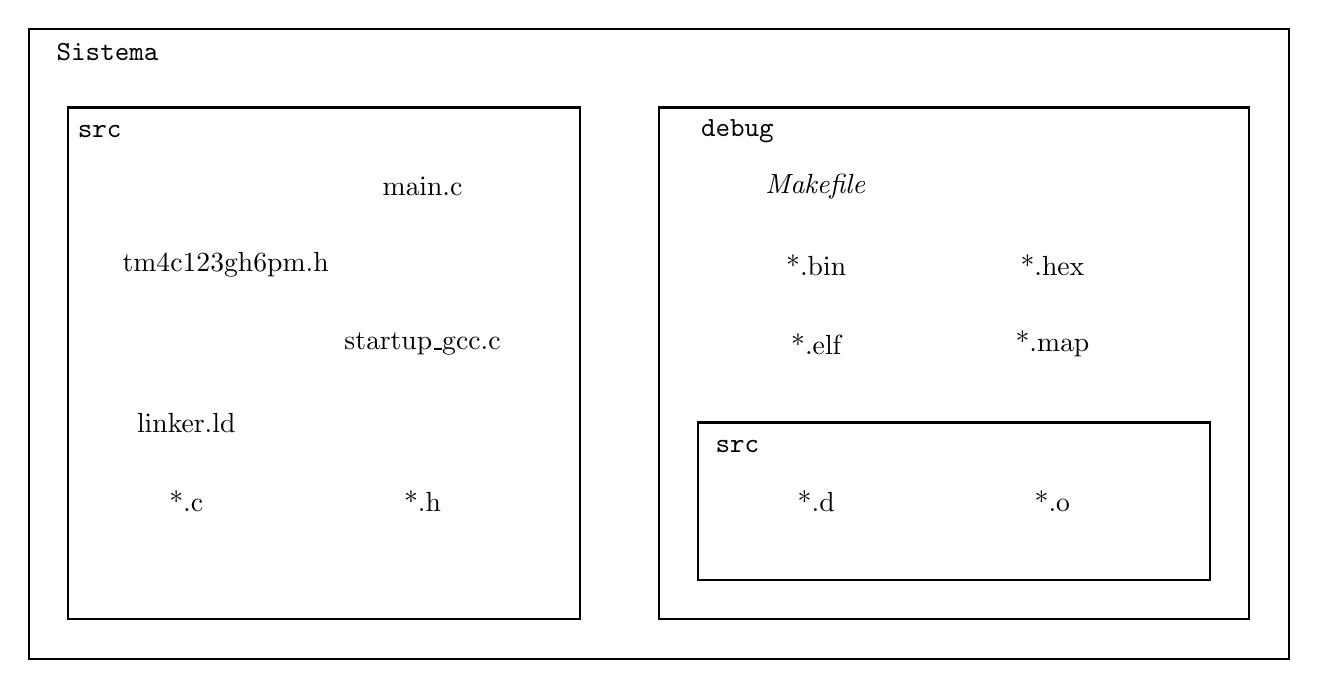
\begin{tikzpicture}[scale=1]
%\draw [lightgray](0,0) grid (16,10);

\draw [black, thick](0,0) rectangle (16, 8); 
\node at (1,7.7) {\textbf{\texttt{Sistema}}};


\draw [black, thick](0.5,0.5) rectangle (7, 7); 
\node at (0.9,6.7) {\textbf{\texttt{src}}};

\node at (5,6) {main.c};
\node at (2.5,5) {tm4c123gh6pm.h};
\node at (5,4) {startup{\_}gcc.c};
\node at (2,3) {linker.ld};
\node at (2,2) {*.c};
\node at (5,2) {*.h};



\draw [black, thick](8,0.5) rectangle (15.5, 7); 
\node at (9,6.7) {\textbf{\texttt{debug}}};

\draw [black, thick](8.5,1) rectangle (15, 3); 
\node at (9,2.7) {\textbf{\texttt{src}}};

\node at (10,6) {\emph{Makefile}};

\node at (10,5) {*.bin};
\node at (13,5) {*.hex};
\node at (10,4) {*.elf};
\node at (13,4) {*.map};
 
\node at (10,2) {*.d};
\node at (13,2) {*.o};

\end{tikzpicture}
\label{fig:estruturaProjeto}

{\small Fonte: Próprio autor}
\end{figure}


Vale um destaque para alguns elementos da estrutura do projeto:


\begin{itemize}
\item Makefile: lista de instruções para automatizar o processo de compilação respeitando a dependecia que deve existir entre arquivos.
\item tm4c123gh6pm.h: arquivo de cabeçalho contendo todas as definições de endereços dos registradores presentes no microcontrolador. Arquivo fornecido pelo fabricante. 
\item startup\_gcc.c: arquivo de inicialização do microcontrolador contendo vetor de interrupção. Arquivo fornecido pelo fabricante.
\item linker.ld: define padrão de disposição de endereços de memória para a família de microcontrolador utilizada. Arquivo utilizado deriva da revisão 14351 da biblioteca TivaWare. 
\item \emph{*.bin}: arquivo binário contendo o programa compilado que é gravado no microcontrolador utilizando o programa \emph{lm4flash}.
\end{itemize}





O projeto foi estruturado basicamente como mostrado na Figura 
\ref{fig:estruturaFirmware}, 
sendo alguns periféricos habilitados e configurados para a 
aplicação como o caso do módulo PWM, 
Interrupções, Temporizador(Timer), 
Comunicação Serial (USART) e \nomenclature{USART}{\emph{Universal Synchronous Receiver Transmitter}}%
pinos de propósito geral (GPIO). \nomenclature{GPIO}{\emph{General Purpose Input/Output}}%
Também foi necessária a implementação de uma Fila 
para armazenamento e cálculo de média.



\begin{figure}[!htb]
\centering
\caption{ Estrutura do Projeto}
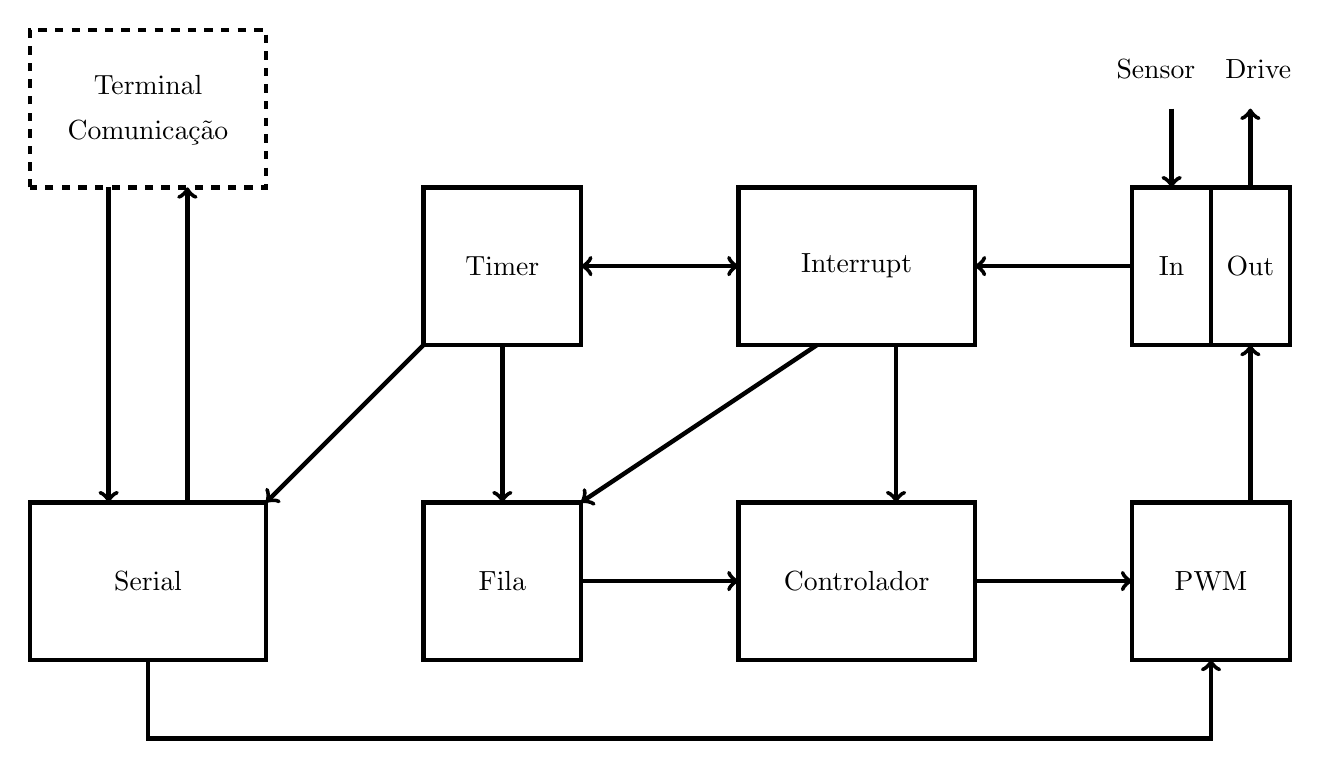
\begin{tikzpicture}[scale=1]
%\draw [lightgray](0,0) grid (16,10);

\draw [black, ultra thick, dashed]( 0,8) rectangle ( 3,10); % terminal de comunicacao
\node at (1.5,9.3){Terminal};
\node at (1.5,8.7){Comunicação};
\draw [ultra thick][->](1,8)--(1,4);
\draw [ultra thick][->](2,4)--(2,8);

\draw [black, ultra thick]( 0,2) rectangle ( 3, 4);  % serial
\node at (1.5,3) {Serial};
\draw [ultra thick][->](1.5,2) -- (1.5,1) -- (15,1) -- (15,2);

\draw [black, ultra thick]( 5,2) rectangle ( 7, 4); % Fila
\node at (6,3) {Fila};
\draw [ultra thick][->](7,3)--(9,3);

\draw [black, ultra thick]( 9,2) rectangle (12, 4); % Controlador
\node at (10.5,3) {Controlador};
\draw [ultra thick][->](12,3)--(14,3);

\draw [black, ultra thick](14,2) rectangle (16, 4); % PWM
\node at (15,3) {PWM};
\draw [ultra thick][->](15.5,4)--(15.5,6);

\draw [black, ultra thick]( 5,6) rectangle ( 7, 8); % Timer
\node at (6,7) {Timer};
\draw [ultra thick][->](6,6)--(6,4);
\draw [ultra thick][->](5,6)--(3,4);
\draw [ultra thick][<->](7,7)--(9,7);

\draw [black, ultra thick]( 9,6) rectangle (12, 8); % Interrupt
\node at (10.5,7) {Interrupt};
\draw [ultra thick][->](11,6)--(11,4);
\draw [ultra thick][->](10,6)--(7,4);

\draw [black, ultra thick](14,6) rectangle (15,8); % In
\node at (14.5,7) {In};
\draw [ultra thick][->](14,7)--(12,7);
\node at (14.3,9.5){Sensor};
\draw [ultra thick][->](14.5,9)--(14.5,8);

\draw [black, ultra thick](15,6) rectangle (16,8); % Out
\node at (15.5,7) {Out};
\draw [ultra thick][->](15.5,8)--(15.5,9);
\node at (15.6,9.5){Drive};

\end{tikzpicture}
\label{fig:estruturaFirmware}

{\small Fonte: Próprio autor}
\end{figure}


O comportamento dos blocos é basicamente o seguinte:

\begin{itemize}

\item \textbf{Timer}: Um temporizador foi configurado para gerar interrupção a cada 10ms. 
Um flag é setado para que a leitura do tempo seja realizada e inserida na fila.
Caso um contador para detectar o tempo de um segundo seja alcançado, o sensor não foi acionado e um zero é adicionado à fila. 
Este contador é reiniciado a cada borda detectada pelo sensor.

\item \textbf{Fila}: Região de memória, com tamanho configurado para uma potência de base 2, para facilitar o cálculo de média. 
A Fila possui um indicador de endereço atual, que contém o último elemento que entrou na Fila, que é o próximo a ser excluído. Assim quanto um dado é inserido na Fila, o valor ocupa a posição do indicador, apagando o dado anterior, e o indicador avança uma posição, até que chegue ao final da Fila e retorne a posição inicial, permanecendo neste círculo infinito, loop. 
Sempre que há a inclusão de um elemento à Fila, o elemento que será excluído é subtraído de uma variável acumulador, em seguida o novo valor é somado ao acumulador e incluído na Fila. 
Após cada inserção de valor no acumulador e na Fila, é feita a divisão do acumulador pela quantidade de posições que a Fila possui, obtendo assim um valor médio. 
A Fila implementada no projeto tem um tamanho de 8 posições. Assim a Fila precisa receber 8 leituras para poder calcular um valor médio consistente. 


\item \textbf{In}: Uma das entradas foi configurada para gerar interrupção a cada borda de subida recebida do elemento sensor, que ocorre a cada giro do eixo do motor. 


\item \textbf{Interrupt}: Rotinas que são executadas somente quando ocorre alguma interrupção, ou seja, quando algum evento esperado ocorre, como no caso de ocorrer uma borda de subida no sensor ou o fim da temporização. 
Em ambos os casos o valor do Timer é lido e escrito na Fila e uma sinalização é gerada no Controlador. 



\item \textbf{Controlador}: Recebe uma sinalização do bloco Interrupt e lê o valor médio da Fila. 
O valor lido é utilizado para realizar os cálculos que estiverem no controladore enviar um sinal adequado ao módulo PWM.


\item \textbf{PWM}: Módulo responsável por receber o valor percentual de atuação em um pino configurado como saída digital. 
Recebe comandos tanto do controlador quando o sistema está operando e realizando efetivamente o controle do processo, quanto do módulo serial, a quem dá prioridade maior para realizar o controle de liga e desliga do sistema. 

\item \textbf{Out}: Basicamente uma das portas (pinos) configurado como Saída Digital que aciona um drive para alimentar o motor.


\item \textbf{Serial}: Módulo que se comunica com o terminal, enviando dados de intervalo de tempo entre interrupções e recebe comando do usuário para iniciar ou parar o processo de controle, ligando ou desligando o módulo PWM.

\item \textbf{Terminal Comunicação}: Módulo que recebe comando para iniciar processo de controle do motor através de interação com o usuário e envia de volta dados de rotação do motor. 
A comunicação é feita através de um programa chamado \emph{minicom};

\end{itemize}


